\subsection{Authentication}

\subsubsection{scope}
\par{This section provides the details use case requirements for the use cases offered by the Authentication
module.}
\begin{figure}[h]
	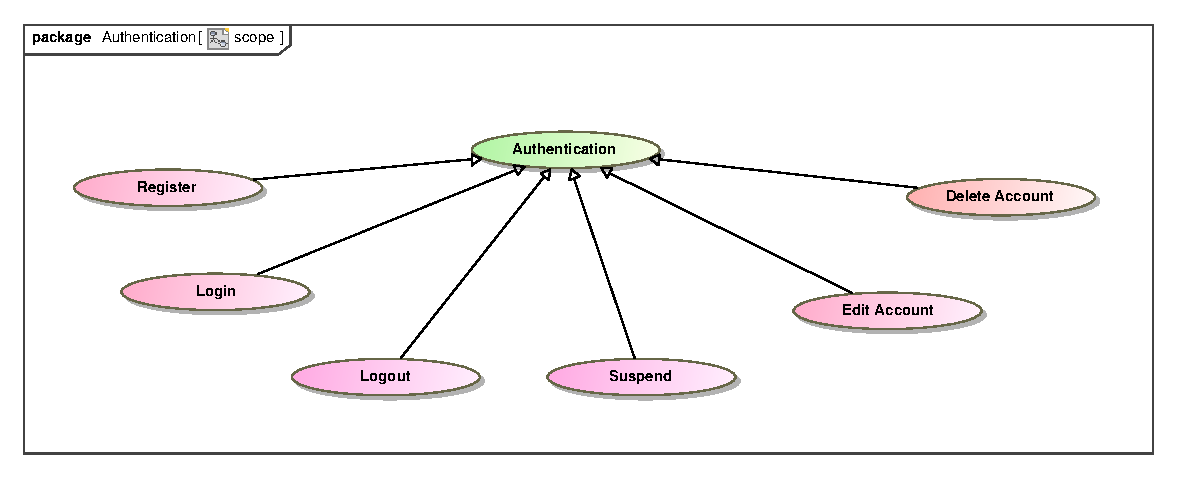
\includegraphics[height=200px, width=500px]{epsImages/Authentication/AuthenticationScope.eps}
	\caption{Scope for authentication module}
\end{figure}

\newpage
\subsubsection{Use Cases}

\begin{enumerate}


\item \textbf{registerAccount  – priority: critical } 
This use case creates  a user account and is persisted through to database.

\par{\textbf{service contract} The service contract for the registerAccount  service is shown in figure below. The pre-conditions are enforced (raising the appropriate exception should they not be met) and the requested account is created and persisted through to database.}

\begin{figure}[h]
		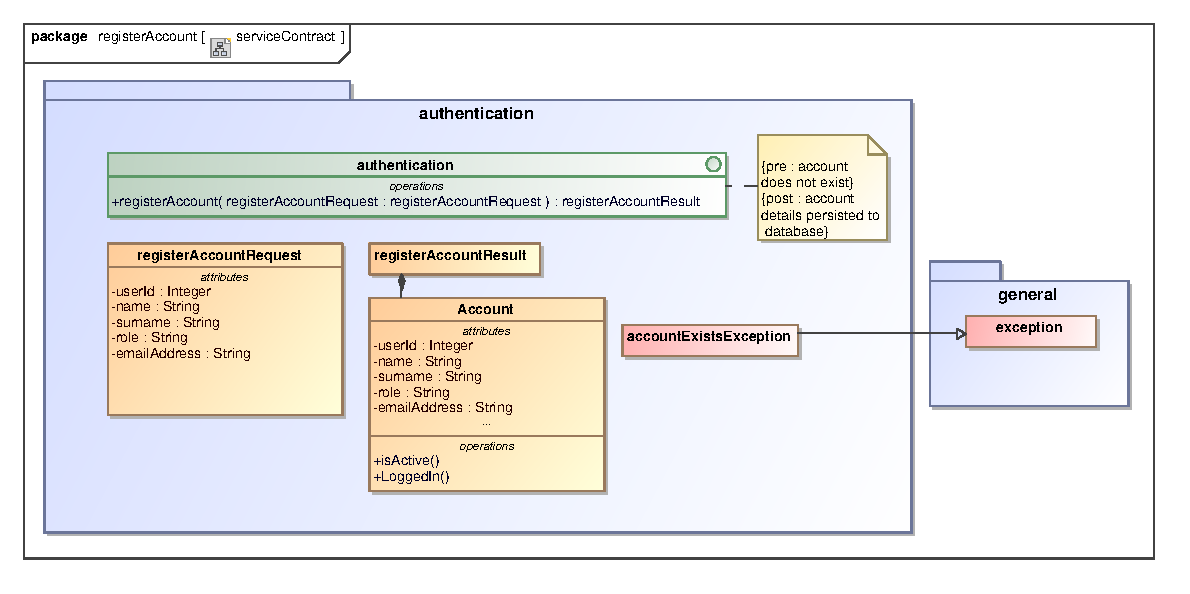
\includegraphics[height=200px, width=500px]{epsImages/Authentication/serviceContract.eps}
		\caption{Service contract for registering new user account}
\end{figure}

\item \textbf{Login - priority: critical}
This use case allows a user to log into an existing account.

\par{\textbf{service contract} The service contract for the login service is shown in figure below.}
\begin{figure}[h]
		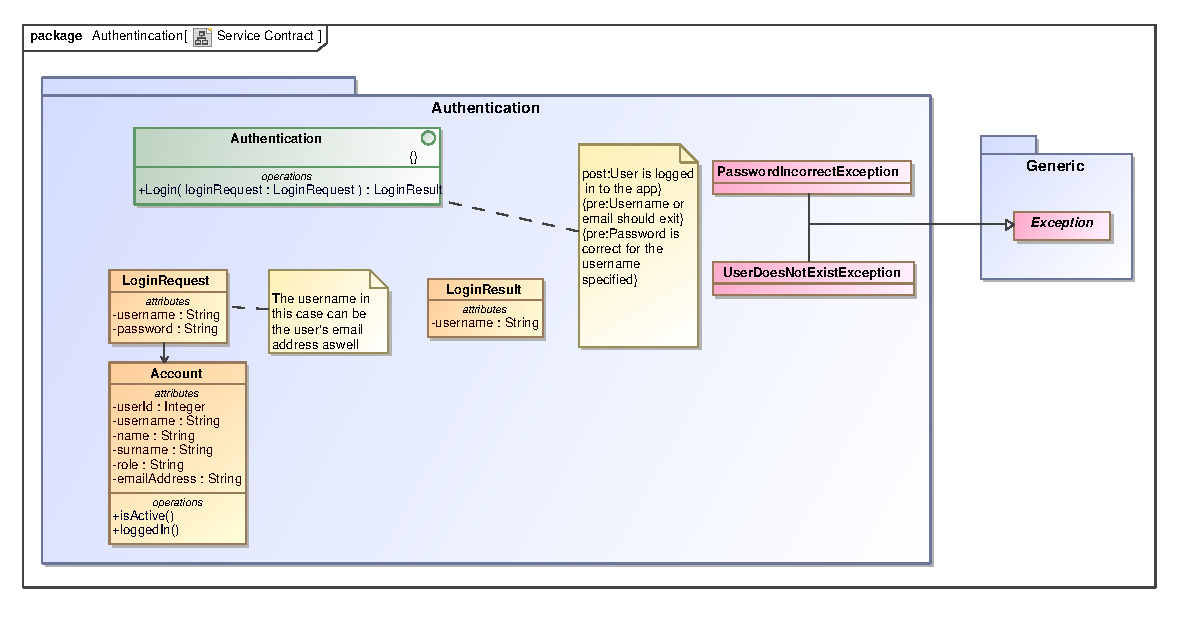
\includegraphics[height=200px, width=500px]{epsImages/Authentication/LoginServiceContract.eps}
		\caption{Service contract for logging into a user account}
\end{figure}

\item \textbf{Logout - priority: important} \\
This use case allows a user to log out of the system safely.

\par{\textbf{Service contract:} The service contract for logging out is shown below. The preconditions are enforced and the users session is ended, thus logging the user out of the system.}
\begin{figure}[h]

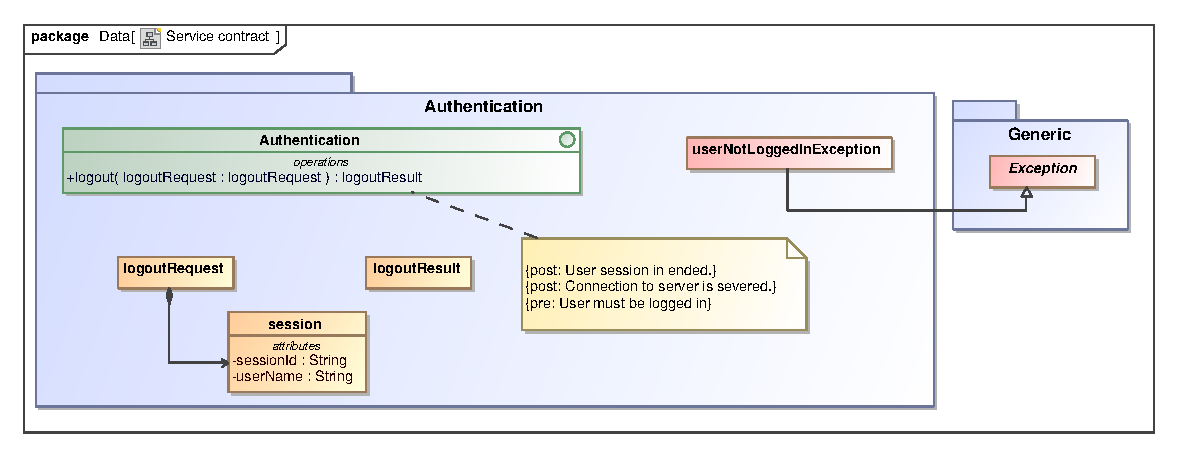
\includegraphics[scale=.9]{epsImages/Authentication/logoutServiceContract.eps}
\caption{Service contract for logging a user out of the system}
\end{figure}
\item \textbf{EditAccount}
\item \textbf{deleteAccount  – priority: important} 
This use case creates  a user account and is persisted through to database.

\par{\textbf{service contract} The service contract for the deleteAccount  service is shown in figure below. The pre-conditions are enforced (raising the appropriate exception should they not be met) and the account of interest is deleted and changes are persisted through to database.}

\begin{figure}[h]
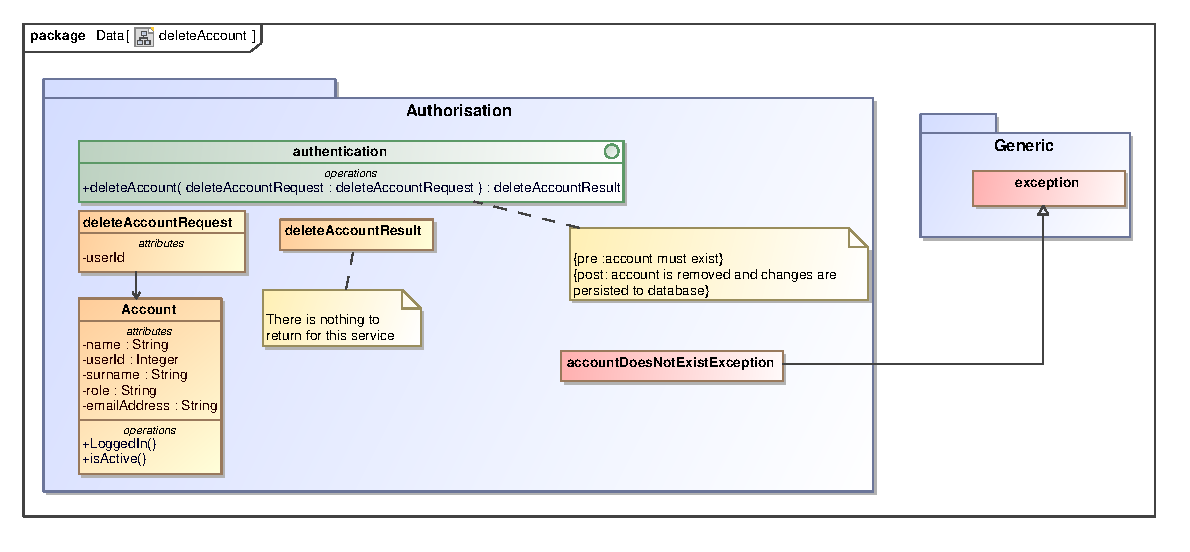
\includegraphics[height=200px, width=500px]{epsImages/Authentication/deleteAccount.eps}
\caption{Service contract for deleting a users account}
\end{figure}
\item \textbf{SuspendAccount - priority: important}\\
This use case allows the system administrator to suspend a users account for any reason he/she may see as appropriate. A suspended account bars the user from logging in and/or using the account until the administrator lifts the suspension.
\\ \textbf{service contract:} The service contract for the suspendAccount service is shown below. 
\begin{figure}[h]
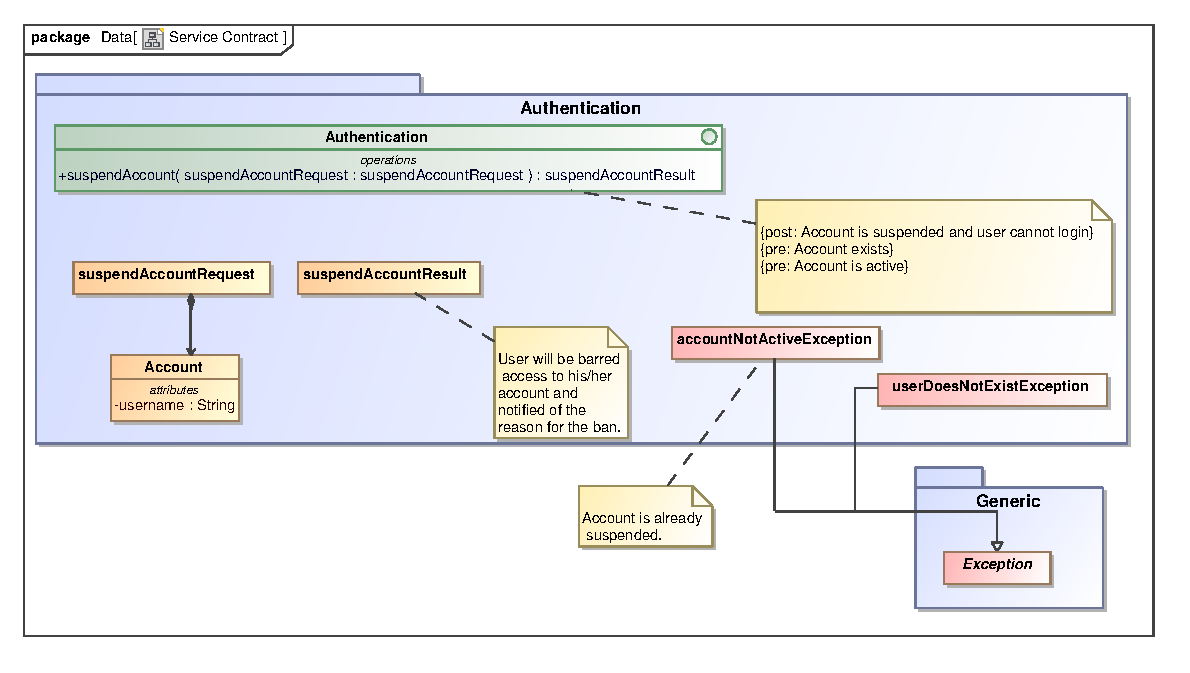
\includegraphics[height=250px, width=500px]{epsImages/Authentication/suspendServiceContract.eps}
\caption{Service contract for suspending a users account}
\end{figure} 
\end{enumerate}
